% (c) 2012 - 2014 Dimitrios Vrettos - d.vrettos@gmail.com
% (c) 2014 Claudio Carboncini - claudio.carboncini@gmail.com
% (c) 2014 Daniele Zambelli - daniele.zambelli@gmail.com

\chapter{Identità, equazioni}

\section{Identità ed equazioni}
\label{sec:13_definizioni}

Analizziamo le proposizioni:

\begin{enumeratea}
\item ``cinque è uguale alla differenza tra sette e due'';
\item ``la somma di quattro e due è uguale a otto'';
\item ``il doppio di un numero naturale è uguale alla differenza tra nove e il 
numero stesso'';
\item ``la somma di due numeri interi è uguale a dieci''.
\end{enumeratea}

Notiamo che sono tutte costruite con il predicato
``essere uguale a''. Riscriviamo in formula ciascuna di esse:
\begin{multicols}{4}
 \begin{enumeratea}
\item $5=7-2$
\item $4+2=8$
\item $2x=9-x$
\item $x+y=10$.
\end{enumeratea}
\end{multicols}
Notiamo che le prime due contengono solamente numeri, le seconde
contengono anche variabili.

Le formule del primo tipo si dicono \emph{chiuse} e
di esse si può subito stabilire se sono vere o false; così in~$\insN$ la
formula~$5 = 7 - 2$ è vera, mentre~$4 + 2 = 8$ è falsa.

\begin{definizione}
 Le \emph{formule chiuse} costruite con il predicato
<<essere uguale>> si chiamano \emph{uguaglianze};
stabilito l'ambiente in cui vengono enunciate si può
immediatamente stabilire il loro valore di verità.
\end{definizione}

\begin{exrig}
 \begin{esempio}
 La formula chiusa~$1 - 6 = -5$ è un'uguaglianza
vera se la consideriamo nell'insieme~$\insZ$ degli interi
relativi, è falsa se la vediamo come sottrazione tra numeri naturali.
 \end{esempio}
\end{exrig}

Le formule c) e d) che contengono variabili si dicono \emph{aperte}; le 
variabili che compaiono sono chiamate
\emph{incognite}. Di tali formule non si può subito stabilire il valore di 
verità.

Quando alle incognite sostituiamo un numero, queste si trasformano in
formule chiuse e allora possiamo stabilirne il valore di verità
relativamente alla sostituzione effettuata.

\begin{exrig}
 \begin{esempio}
 Nella formula~$2x = 9 - x$ sostituiamo alla variabile~$x$ il valore $0$ 
otteniamo:~$2\cdot 0=9-0 \Rightarrow~0=9$, falsa.

 Sostituiamo ora alla
variabile~$x$ il valore $3$ otteniamo~$2\cdot 3=9-3 \Rightarrow~6=6$, vera.
 \end{esempio}

 \begin{esempio}
 Nella formula~$x + y = 10$ sostituiamo
alle variabili coppie di numeri interi come~$x = 2$ e~$y = 5$ 
otteniamo~$2+5=10\Rightarrow~7= 10$, falsa. Se
sostituiamo~$x = 4$ e~$y = 6$ ci rendiamo subito conto che
l'uguaglianza ottenuta è \emph{vera}. Esistono
molte altre coppie di numeri interi rendono vera
l'uguaglianza.
 \end{esempio}
\end{exrig}

\begin{definizione}
 Le formule aperte costruite con il predicato essere uguale si chiamano
\emph{equazioni}; le due espressioni che compaiono a sinistra e a
destra del segno di uguaglianza si chiamano rispettivamente
\emph{primo membro} e \emph{secondo membro}.

L'insieme dei valori che sostituiti alle incognite trasformano l'equazione in
un'uguaglianza vera costituisce
l'\emph{insieme soluzione} ($\IS$) o più semplicemente la \emph{soluzione} 
dell'equazione.
\end{definizione}

Affronteremo per ora equazioni in
\emph{una sola incognita} che, dopo aver svolto eventuali calcoli nei due 
membri, comparirà a
\emph{grado} 1 e i cui \emph{coefficienti} sono \emph{numeri razionali}.
Cercheremo la sua soluzione
nell'insieme~$\insQ$ dei numeri razionali, salvo esplicita indicazione 
differente.
\begin{exrig}
 \begin{esempio}
Cercare le soluzioni nell'insieme indicato.
 \begin{enumeratea}
 \item $x^{2}=1 \text{ con }x\in\insN.$
Risulta vera solo se a~$x$ sostituiamo il valore~1; infatti~1 è
l'unico numero naturale il cui quadrato è~1.
L'insieme soluzione è~$\{1\}$.
 \item $x^{2}=1 \text{ con }x\in\insZ$.
Risulta vera se a
$x$ sostituiamo il valore~1 oppure il valore~$-1$ infatti sia~$-1$ che~1
elevati al quadrato danno~1. L'insieme soluzione è
$\{-1, 1\}$.
 \item $x^{2}+1=0\text{ con }x\in\insR$.
Essendo la formula a sinistra
dell'uguale la somma di un quadrato con il numero~1, si ottiene sempre
un numero~$\geq1$ e non si può ottenere $0$, pertanto è impossibile trovare una 
soluzione.
 \item $2x+3=(3+x)+x \text{ con } x\in\insQ$.
Eseguendo il semplice calcolo al secondo
membro, ci rendiamo conto che qualunque valore venga sostituito
all'incognita l'uguaglianza risulta
vera. L'insieme soluzione è~$\insQ$.
\end{enumeratea}
 \end{esempio}
\end{exrig}

In generale un'equazione in una incognita può essere:

\begin{enumeratea}
\item \emph{determinata}, quando l'insieme soluzione è un sottoinsieme proprio
dell'insieme numerico considerato;
\item \emph{impossibile}, quando l'insieme soluzione è l'insieme 
vuoto~$\emptyset$
\item \emph{indeterminata} o \emph{identità}, quando l'insieme soluzione 
coincide con
l'insieme considerato.
\end{enumeratea}

\begin{exrig}
 \begin{esempio}
 Analizziamo le equazioni:
\begin{multicols}{3}
 \begin{enumeratea}
 \item $3\cdot x=0$
 \item $0\cdot x=5$
 \item $0\cdot x=0$.
\end{enumeratea}
\end{multicols}

Tutte e tre hanno la stessa struttura: il primo membro è il prodotto
di un coefficiente numerico per un valore incognito, il secondo membro
è un numero.

\paragraph{a)} Per trovare l'insieme soluzione della prima equazione cerchiamo 
in~$\insQ$ il
numero che moltiplicato per~3 dà come prodotto~0. L'unico numero che rende vera
l'uguaglianza è zero. Quindi l'insieme delle soluzioni è~$\{0\}$. L'equazione è
determinata.

\paragraph{b)} Per trovare l'insieme soluzione della seconda equazione cerchiamo 
in~$\insQ$ il
numero che moltiplicato per~0 dà come prodotto~5. Per la proprietà
della moltiplicazione quando moltiplichiamo per~0 il prodotto è~0,
non otterremo mai~5. Quindi l'insieme soluzione è
l'insieme vuoto. L'equazione è
impossibile.

\paragraph{c)} Per trovare l'insieme soluzione della terza equazione cerchiamo 
in~$\insQ$ il
numero che moltiplicato per zero dà come prodotto zero. Per la
proprietà della moltiplicazione quando moltiplichiamo per~0 il
prodotto è~0 qualunque sia l'altro fattore. Quindi
l'insieme delle soluzioni è~$\insQ$. L'equazione è
indeterminata.
 \end{esempio}
\end{exrig}

\subsection{Ricerca dell'insieme soluzione}
In alcuni casi la soluzione di un'equazione si può
trovare applicando semplicemente le proprietà delle operazioni.

\begin{exrig}
 \begin{esempio}
Analizziamo lo schema operativo dell'equazione~$3x-1=17 \text{ con } x\in\insN$.

Si opera sul valore incognito~$x$ per ottenere~17:

\[\text{\emph{entra} } x,\text{ si moltiplica per tre}\to~3\cdot x%
\text{ si sottrae } 1\to~3\cdot x-1 \text{ si ottiene } 17.\]

Qual è il valore in ingresso?

Per determinare il valore in ingresso basterà ripercorrere lo schema
 effettuando le operazioni inverse:
\[\text{\emph{da} } 17 \text{ aggiungi } 1\to~18 \text{ dividi per tre }\to~18:3 
\to x.\]

La soluzione dell'equazione è~$x = 6$ e~$\IS$ (insieme
soluzione) è~$\{6\}$.
 \end{esempio}
\end{exrig}

% \ovalbox{\risolvi \ref{ese:13.1}}\vspace{1.10ex}

Per risolvere un'equazione più complessa come
$\left(\dfrac{1}{2}x+3\right)\cdot (-5+x)=12x+\dfrac{1}{2}x^{2}$ con
$x\in~\insQ$, non possiamo applicare il procedimento precedente; potremmo
procedere per tentativi, sostituendo all'incognita
alcuni valori scelti a caso e verificando se il valore assunto dal
primo membro risulta uguale a quello assunto dal secondo membro. È
evidente però che questo procedimento raramente porterà a trovare
tutte le soluzioni di un'equazione.

\osservazione
Per risolvere un'equazione, cioè per determinare tutte
le eventuali soluzioni, si procede applicando i principi
d'equivalenza.

\section{Prinicipi di equivalenza}
\label{sec:13_principi}

\begin{definizione}
 Due equazioni sono \emph{equivalenti} se hanno lo stesso insieme soluzione.
\end{definizione}

\begin{principio}[Primo principio di equivalenza]
 Aggiungendo o sottraendo ad ambo i membri di
un'equazione data uno stesso numero o una stessa
espressione (definita per ogni valore dell'incognita)
si ottiene un'equazione equivalente a quella data.
\end{principio}

\begin{principio}[Secondo principio di equivalenza]
 Moltiplicando o dividendo ambo i membri di
un'equazione per uno stesso numero non nullo o per
un'espressione non nulla (definita per ogni valore
attribuito all'incognita) si ottiene
un'equazione equivalente alla data.
\end{principio}


La forma più semplice di un'equazione di primo grado in
un'incognita è del tipo:
\[x = \text{ numero}.\]

L'insieme soluzione di una
equazione di questo tipo è semplicemente:
\[\IS=\{\text{ numero} \}.\]

Per esempio, l'insieme delle soluzioni dell'equazione
$x = -3$ è~$\IS =\{-3\}$.

I principi sopra enunciati permettono di trasformare qualunque equazione
nella forma canonica che ha lo stesso insieme soluzione di quella
assegnata.

\subsection{Risoluzione di equazioni numeriche intere di primo grado}
In questo paragrafo vedremo come usare i principi
d'equivalenza prima enunciati per condurre
un'equazione alla forma canonica e dunque determinarne
la soluzione.

\begin{definizione}
Risolvere un'equazione significa
determinare il suo Insieme Soluzione.
\end{definizione}

Cominciamo con alcuni esempi.

\begin{exrig}
 \begin{esempio}
Applicazione del~1{\textdegree} principio di equivalenza.

\begin{enumeratea}
\item $x-5=3$:
aggiungiamo~5 a entrambi i membri:~$x-5+5=3+5\Rightarrow x=8$, $\IS =\{8\}.$
\item $3x=2+2x$: sottraiamo~$2x$ a entrambi i membri:~$3x-2x=2+2x-2x\Rightarrow 
x=2$,
$\IS =\{2\}$.
\end{enumeratea}
 \end{esempio}

% \ovalbox{\risolvii \ref{ese:13.2}, \ref{ese:13.3}, \ref{ese:13.4}, 
% \ref{ese:13.5}}

 \begin{esempio}
 Applicazione del~2{\textdegree} principio di equivalenza.

 \begin{enumeratea}
\item $3x=12$ dividiamo entrambi i membri per~3, si ha
\[\dfrac{3}{3}x=\dfrac{12}{3}\Rightarrow x=4\to\IS =\{4\}.\]
\item $\dfrac{1}{2}x=2$ moltiplichiamo entrambi i membri per~2, si ha
\[2\cdot {\dfrac{1}{2}}x=2\cdot 2\Rightarrow x=4\to\IS =\{4\}.\]
\end{enumeratea}
\end{esempio}

% \ovalbox{\risolvii \ref{ese:13.6}, \ref{ese:13.7}, \ref{ese:13.8}}

% \newpage
 \begin{esempio}
 $-2x+1=3x-5$.

\begin{enumeratea}
 \item Sottraiamo~1 a entrambi i membri~$-2x+1-1=3x-5-1$ quindi~$-2x=3x-6$
\item sottraiamo~$3x$ a entrambi i membri~$-2x-3x=3x-3x-6$ quindi~$-5x=-6$
\item dividiamo entrambi i membri 
per~$-5$:~$\dfrac{-5}{-5}x=\dfrac{-6}{-5}\Rightarrow x=\dfrac{6}{5}\rightarrow
\IS =\left\{\dfrac{6}{5}\right\}.$
\end{enumeratea}
 \end{esempio}

% \ovalbox{\risolvii \ref{ese:13.9}, \ref{ese:13.10}, \ref{ese:13.11}}
 \begin{esempio}
Prendiamo l'equazione~$(x+1)+3\cdot (2+x)=12x-1$ nella
sola incognita~$x$ di primo grado a coefficienti numerici interi.
Cerchiamo di trasformarla nella forma canonica ``$x =$
numero'' applicando i principi di equivalenza.

\begin{enumerate}
 \item svolgiamo i calcoli al primo e al secondo
membro:~$x+1+6+3x=12x-1$.
 \item sommiamo in ciascun membro i termini
simili (se ce ne sono):~$4x+7=12x-1$.
 \item sottraiamo ad ambo i membri il monomio~12x, 
 applicando il primo principio:~$4x-12x+7=12x-1-12x$, sommiamo i
monomi simili al primo e al secondo membro e otteniamo~$-8x+7=-1$.
 \item sottraiamo ad ambo i membri il numero~7,
applicando il primo principio e sommiamo i termini simili:
$-8x+7-7=-1-7\Rightarrow -8x=-8$.
 \item dividiamo ambo i membri per~$-8$,
applicando il secondo principio:
$\dfrac{-8}{-8}x=\dfrac{-8}{-8}\Rightarrow x=1$.
\end{enumerate}

L'equazione assegnata~$(x+1)+3\cdot (2+x)=12x-1$
risulta equivalente all'ultima trovata x=1, pertanto il
suo insieme soluzione è~$\IS = \{1\}$.
 \end{esempio}
\end{exrig}

% \vspace{1.10ex}% \ovalbox{\risolvii \ref{ese:13.12}, \ref{ese:13.13}}

\osservazione
La trasformazione di un'equazione nella forma canonica
prevede che il termine con l'incognita sia collocato da
una parte del segno uguale mentre dall'altra parte sia
posto il termine numerico.

Enunciamo alcune \emph{regole pratiche} che ci possono aiutare nella
procedura risolutiva e che discendono direttamente dal primo principio
d'equivalenza.

\paragraph{a)} Spostando da un membro all'altro un addendo occorre
cambiargli il segno; l'equazione ottenuta è
equivalente a quella data.

$2x-3=2$, per lasciare da sola la~$x$ al primo menbro devo aggiungere~$+3$ al 
primo e
al secondo membro, ottengo~$2x-3+3=2+3$ da cui~$2x=2+3$.

L'effetto che si ha è che si è spostato il~$-3$ al
secondo membro cambiandolo di segno.

\paragraph{b)} Se in entrambi i membri dell'equazione compare uno
stesso addendo con lo stesso segno, esso può essere cancellato da
entrambi i membri: l'equazione che si ottiene è
equivalente a quella data.

Infatti:
$2x-3+x=2+x$. La~$x$ che sta al secondo membro va portata al primo, cambiandola 
di segno
$2x-3+x-x=2$ da cui~$2x-3=2$.

L'effetto che si ha è che si possono eliminare le due
x che stanno una al primo membro e una al secondo membro.


\paragraph{c)} Se il coefficiente dell'incognita è~$-1$, %ossia
l'equazione si presenta nella forma~$-x=n$, si
può cambiare di segno ai termini del primo e del secondo membro, per
ottenere la forma~$x=-n$. Cambiare di segno equivale a moltiplicare per
$-1$ i due membri dell'equazione.

Infatti:

$x-3=2x+1$. Dobbiamo portare~$2x$ al primo membro e~$-3$ al secondo membro, 
otteniamo
$x-2x=3+1$ da cui~$-x=4$.

Poiché il coefficiente della x è negativo moltiplichiamo per~$-1$
primo e secondo membro
$-1\cdot (-x)=-1\cdot (4)$ da cui~$x=-4$.

\begin{problema}
 Risolvi la seguente equazione applicando queste regole pratiche.
 \[5x+2\cdot (3-x)+1=-(4x-1)+2\cdot (6-x).\]
\end{problema}

\begin{soluzione}
I passi da effettuare sono
\begin{enumerate}
 \item svolgiamo i calcoli:~$5x+6-2x+1=-4x+1+12-2x$
 \item eliminiamo i termini uguali che compaiono nei due membri:
 \[5x+6 \cancel{-2x}\cancel{+1}=-4x 
\cancel{+1}+12\cancel{-2x}\Rightarrow~5x+6=-4x+12;\]
 \item spostiamo il monomio~$-4x$ del secondo membro a sinistra del segno uguale 
e il numero~$+6$
da sinistra a destra, ottenendo:~$5x+4x=-6+12$
\item sommando i termini simili nei due membri, otteniamo~$9x=+6$ da cui 
dividendo per nove
 ambo i membri si ottiene
 \[x=\dfrac{2}{3}\to \IS =\left\{\dfrac{2}{3}\right\}.\]
 \end{enumerate}

\end{soluzione}
% \ovalbox{\risolvii \ref{ese:13.14}, \ref{ese:13.15}, \ref{ese:13.16}, 
% \ref{ese:13.17}, \ref{ese:13.18}}

\section{Equazioni a coefficienti frazionari}
\label{sec:13_coefffraz}

Vediamo, illustrando qualche esempio, come si procede.

 \begin{esempio}
$\dfrac{2}{3}x+4-\dfrac{1}{2}+2x=\dfrac{x+2}{3}-\dfrac{5}{2}x+1$.

Sappiamo che il secondo principio d'equivalenza ci
permette di moltiplicare ambo i membri per uno stesso numero diverso da
zero per ottenere un'equazione equivalente alla data.

\begin{enumerate}
 \item Calcoliamo il~$\mcm$ tra i denominatori: in questo
caso~$\mcm$(2,3) = 6
 \item Moltiplichiamo per~6 ambo i membri
dell'equazione:
\[6\left(\dfrac{2}{3}x+4-\dfrac{1}{2}+2x\right)=6\left(\dfrac{x+2}{3}-\dfrac{5}{
2}x+1\right).\]
 \item Eseguiamo i calcoli:~$4x+24-3+12x=2x+4-15x+6$.
\end{enumerate}

I coefficienti dell'equazione sono ora numeri interi,
puoi procedere da solo come abbiamo visto negli esempi precedenti. Il risultato 
è $x=-\dfrac{11}{25}$.
\end{esempio}

% \ovalbox{\risolvi \ref{ese:13.19}}

\subsection{Equazioni in cui l'incognita compare con grado maggiore di~1}

% \begin{exrig}\vspace{1.10ex}
 \begin{esempio}

$(2x+1)\cdot (x-2)=2\cdot (x+1)^{2}-5x$.

Prima di iniziare la procedura risolutiva analizziamo i membri
dell'equazione: al primo membro compare il prodotto
di due polinomi di primo grado, nel secondo il quadrato di un binomio
di primo grado, pertanto l'incognita comparirà a grado due. Apparentemente
l'equazione è di secondo grado. Iniziamo la procedura
risolutiva:

\begin{enumerate}
 \item svolgiamo i calcoli e otteniamo:
$2x^{2}-4x+x-2=2x^{2}+4x+2-5x\Rightarrow~2x^{2}-3x-2=2x^{2}-x+2.$
 \item applichiamo le regole pratiche eliminando i monomi
uguali con l'incognita al secondo grado e otteniamo
$-3x+x=+2+2$.

Abbiamo ottenuto un'equazione di primo grado; puoi
procedere da solo e determinare la forma canonica e~$\IS$.
 \item \dotfill
\end{enumerate}

 \end{esempio}

% \end{exrig}


\subsection{Equazioni in cui l'incognita scompare}

% \begin{exrig}\vspace{1.10ex}
 \begin{esempio}
 $\dfrac{4}{5}-\dfrac{x}{2}=\dfrac{2-5x}{10}$.

 \begin{enumerate}
  \item Calcoliamo il~$\mcm$ tra i denominatori: in questo
caso~$\mcm(5, 2, 10) = 10$.
  \item Moltiplichiamo per~10 ambo i membri
dell'equazione:
$10\left(\dfrac{4}{5}-\dfrac{x}{2}\right)=10\left(\dfrac{2-5x}{10}\right)$.
  \item Eseguiamo i calcoli:~$8-5x=2-5x$.
  \item Applichiamo la regola pratica:
$-5x+5x=2-8$ i monomi in~$x$ si annullano!
  \item Sommando i monomi simili si ottiene:~$0\cdot x=-6$.
 \end{enumerate}

Il coefficiente dell'incognita è zero; non possiamo
applicare il secondo principio e dividere ambo i membri per zero.
D'altra parte non esiste nessun numero che moltiplicato
per zero dia come prodotto~$-6$. Quindi~$\IS =\emptyset $,
l'equazione risulta impossibile.
 \end{esempio}

 \begin{esempio}
$\dfrac{x}{6}-\dfrac{2x}{3}=-{\dfrac{x}{2}}$.

\begin{enumerate}
 \item Calcoliamo il~$\mcm$ tra i denominatori: in questo
caso~$\mcm(6, 3, 2) = 6$.
 \item Moltiplichiamo per~6 ambo i membri
dell'equazione:
$6\left(\dfrac{x}{6}-\dfrac{2x}{3}\right)=6\left(-{\dfrac{x}{2}}\right)$.
 \item Eseguiamo i calcoli:~$x-4x=-3x$.
 \item Applicando il primo principio si ottiene~$0\cdot x=0$.
\end{enumerate}

Il coefficiente dell'incognita è zero; non possiamo
applicare il secondo principio e dividere ambo i membri per zero.
D'altra parte per la proprietà della moltiplicazione
qualunque numero moltiplicato per zero dà come prodotto zero. Quindi
$\IS = \insQ$, l'equazione è indeterminata (identità).
 \end{esempio}

% \end{exrig}

\subsection{Riassunto}
$A\cdot x=B$ con~$A$ e~$B$ numeri
razionali è la forma canonica dell'equazione di primo grado in una
incognita a coefficienti numerici.% è $A\cdot x=B$ con~$A$ e~$B$ numeri
%razionali.

Possono presentarsi i casi:
 \begin{itemize*}
 \item se~$A\neq~0$ possiamo applicare il secondo principio
d'equivalenza dividendo ambo i membri per~$A$ quindi
$\IS =\left\{\dfrac{B}{A}\right\}$. L'equazione
è determinata.

 \item se~$A=0$ non possiamo applicare il secondo principio
d'equivalenza e dividere ambo i membri per~$A$ e si
presentano due casi:

\begin{itemize*}
 \item $B=0$ allora~$\IS =\insQ$. L'equazione
è indeterminata.

\item $B\neq~0$ allora~$\IS =\emptyset $.
L'equazione è impossibile.
\end{itemize*}


 \end{itemize*}

Lo schema precedente si può rappresentare anche con un grafo ad
albero:
\begin{center}
 % (c) 2012 -2013 Dimitrios Vrettos - d.vrettos@gmail.com

\begin{tikzpicture}[x=5mm, y=5mm,font=\small]
\tikzstyle{level 1}=[level distance=2cm, sibling distance=2.cm]
\tikzstyle{level 2}=[level distance=2cm, sibling distance=1.cm]
\tikzstyle{point} = [circle,minimum width=3pt,fill, inner sep=0pt]

\node[point, label=left:{$A\cdot x =B$}] (aer) at (0,0) {}[grow'=right]
child {node[point, label=right:{$A\ne 0\to$ equazione determinata e $\IS=\left\{\dfrac{B}{A}\right\}$}] {} 
}
child {node[point, label=below:{$A=0$}] {} 
child {node[point,label=right:{$B=0\to$ equazione indeterminata e $\IS=\insQ$}] {}}
child {node[point,label=right:{$B\ne 0\to$ equazione impossibile e $\IS=\emptyset $}] {}}
} ;
\end{tikzpicture}
\end{center}

% \ovalbox{\risolvii \ref{ese:13.20}, \ref{ese:13.21}, \ref{ese:13.22}, 
% \ref{ese:13.23}, \ref{ese:13.24}, \ref{ese:13.25}, \ref{ese:13.26}, 
% \ref{ese:13.27}, \ref{ese:13.28}, \ref{ese:13.29},
% \ref{ese:13.30}}

% \ovalbox{\ref{ese:13.31}, \ref{ese:13.32}, \ref{ese:13.33}, \ref{ese:13.34}, 
% \ref{ese:13.35}, \ref{ese:13.36}, \ref{ese:13.37}, \ref{ese:13.38}, 
% \ref{ese:13.39},
% \ref{ese:13.40}, \ref{ese:13.41}, \ref{ese:13.42}, \ref{ese:13.43}, 
% \ref{ese:13.44}}

% \ovalbox{\ref{ese:13.45}, \ref{ese:13.46}, \ref{ese:13.47}, \ref{ese:13.48}, 
% \ref{ese:13.49},\ref{ese:13.50}}


\section{Problemi di I grado in un'incognita}
\label{sec:equazioni_problemi}

\subsection{Un po' di storia e qualche aneddoto}
\label{subsec:equazioni_problemi_storia}

Sin dall'antichità l'uomo si è
trovato di fronte a difficoltà pratiche, legate alla vita quotidiana
e ha perciò messo a punto strategie per superarle.

Sembra che nell'antico Egitto le periodiche piene del
Nilo abbiano spinto l'uomo a sviluppare la capacità
di tracciare rette parallele, rette perpendicolari, di misurare il
perimetro e l'area di particolari figure geometriche o
viceversa di calcolare le misure dei lati di poligoni di dato perimetro
o data area per poter ridefinire i confini degli appezzamenti di
terreno.

Il \emph{papiro di Rhind}
\footnote{Dal nome dell'inglese A.~H.~Rhind che lo comprò a Luxor nel~1858.}, 
testo egizio scritto in
ieratico, risalente al~1700~\aC, si autodefinisce
``istruzioni per conoscere tutte le cose
oscure'' contiene più di~85 problemi con relativi
metodi di soluzione riguardanti il calcolo della capacità di
recipienti e di magazzini, la ricerca dell'area di
appezzamenti di terreno e altre questioni aritmetiche.

Nel problema~24 del papiro, ad esempio, viene calcolato il mucchio
quando esso ed il suo settimo sono uguali a~19. Mucchio è
l'incognita del problema, indicata con il termine
\emph{aha} il cui segno è
% % (c) 2012 Dimitrios Vrettos - d.vrettos@gmail.com
\begin{hieroglyph}{\leavevmode \loneSign{{\Hsmaller\Aca GD/66/}}}\end{hieroglyph}.

\begin{inaccessibleblock}[Geroglifico]
 
\includegraphics[scale=0.28]{img/giero.png}.
\end{inaccessibleblock}
                                                                  
Noi traduciamo la richiesta nell'equazione~$x+\dfrac{1}{7}x=19$.

Nel~1202 Leonardo Pisano, conosciuto col nome paterno di
`filius Bonacci' o Fibonacci, pubblicò il
\emph{Liber Abaci} in cui, a partire dall'ottavo
capitolo, presenta vari metodi algebrici per la risoluzione di problemi
di matematica applicata, legati alla realtà
dell'epoca, in particolare
all'ambiente commerciale. I nuovi
``algoritmi'' presentati da Fibonacci,
intendevano facilitare la risoluzione dei problemi di calcolo evitando
l'utilizzo dell'abaco. Nel~1223 a
Pisa, l'imperatore Federico~II di Svevia, assistette a
un singolare torneo tra matematici dell'epoca; il
problema proposto era il seguente:

<<Quante coppie di conigli si ottengono in un anno (salvo i
casi di morte) supponendo che ogni coppia dia alla luce
un'altra coppia ogni mese e che le coppie più
giovani siano in grado di riprodursi già al secondo mese di
vita?>>.

Fibonacci vinse la gara dando al quesito una risposta così rapida da
far persino sospettare che il torneo fosse truccato. La soluzione fu
trovata tramite l'individuazione di una particolare
successione di numeri, nota come successione di Fibonacci.

Secondo la leggenda, il grande matematico Carl Fiedrich Gauss già
all'età di tre anni avrebbe corretto un errore di
suo padre nel calcolo delle sue finanze. All'età di
10 anni fu autorizzato a seguire le lezioni di aritmetica di un certo
Buttner. Un giorno, agli studenti particolarmente turbolenti, Buttner
diede come compito di punizione il calcolo della somma dei primi~100
numeri, da~1 a~100. Poco dopo, sorprendendo tutti, il giovanissimo Carl
diede la risposta esatta, ``5050''.
Si era accorto che mettendo in riga tutti i numeri da~1 a~100 e nella
riga sottostante i numeri da~100 a~1, ogni colonna dava come somma~101;
fece dunque il prodotto~$100\times~101$ e divise per~2, ottenendo facilmente il
risultato: Buttner rimase sgomento.

\subsubsection{Risoluzione dei problemi}

 \epigraph{La risoluzione dei problemi \ldots serve ad acuire
 l'ingegno e a dargli la facoltà di penetrare
 l'intera ragione di tutte le cose.}{{\scshape{R. Descartes}}}

I problemi che possono presentarsi nel corso degli studi o
nell'attività lavorativa sono di diversa natura: di
tipo economico, scientifico, sociale, possono riguardare insiemi
numerici o figure geometriche. La matematica ci può aiutare a
risolvere i problemi quando essi possono essere tradotti in
``forma matematica'', quando cioè
è possibile trascrivere in simboli le relazioni che intercorrono
tra le grandezze del problema.

Analizzeremo problemi di tipo algebrico o geometrico, che potranno
essere formalizzati attraverso equazioni di primo grado in una sola
incognita. Prima di buttarci alla risoluzione del problema, procediamo a:

\begin{enumeratea}
\item una lettura ``attenta'' del
testo al fine di individuare l'ambiente del problema,
le parole chiave, i dati e le informazioni implicite,
l'obiettivo;
\item la scelta della grandezza incognita e la descrizione
dell'insieme in cui si ricerca il suo valore,
ragionando sull'obiettivo del problema (condizioni sull'incognita);
\item la traduzione in ``forma matematica'' delle relazioni che intercorrono 
tra i dati e l'obiettivo, cioè l'individuazione dell'equazione risolvente;
\item la risoluzione dell'equazione trovata;
\item il confronto tra la soluzione trovata e le condizioni poste su di essa.
\end{enumeratea}

\begin{problema}
 Un mattone pesa un chilo più mezzo mattone. Quanto pesa un mattone?
\end{problema}

\begin{soluzione}
 La situazione può essere materialmente descritta con una figura.
Togliamo da ogni piatto della bilancia mezzo mattone, la bilancia è
ancora in equilibrio come mostra la figura~2, da ciò possiamo
dedurre che mezzo mattone pesa un chilo. Il mattone intero pesa dunque
due chili.
\begin{center}
 % (c) 2012 Dimitrios Vrettos - d.vrettos@gmail.com
\begin{tikzpicture}[font=\small,x=5mm, y=5mm, scale=.75]

\begin{scope}[fill=black, draw=black]
\filldraw (0,0) rectangle (4,1);
\filldraw[rounded corners=2] (1,1.1)rectangle (3,1.6);
\filldraw (1.8,1.7) rectangle (2.3,8);
\filldraw[rounded corners=2] (1.5,8.1)rectangle (2.6,8.6);
\filldraw (-4,8.7) rectangle (8,9.1);
\filldraw[rounded corners=2] (1.8,8.8)rectangle (2.3,9.8);

\node[name=c1,shape=semicircle,shape border rotate=180, inner sep=3.75mm,draw=black, fill=black] at (-4,3)
{};
\node (a) at (-4,8.7) {};
\draw (a.center)--(c1.arc start);
\draw (a.center)--(c1.arc end);

\node[name=c2,shape=semicircle,shape border rotate=180, inner sep=3.75mm,draw=black, fill=black] at (8,3)
{};
\node (b) at (8,8.7) {};
\draw (b.center)--(c2.arc start);
\draw (b.center)--(c2.arc end);

\filldraw[fill=orange, draw=orange](-5.5,4.02) rectangle (-2.5,5.1);
\filldraw[fill=orange, draw=orange](6.5,4.02) rectangle (8,5.1);
\filldraw[fill=white] (8.3,4) rectangle (9.7,5.1);
\filldraw[fill=white] (8.6,5.1) rectangle (9.4,5.4);
\node () at (9,4.5) {1kg};
\node () at (2,-1) {Figura 1};
\end{scope}

\begin{scope}[fill=black, draw=black, xshift=100mm]
\filldraw (0,0) rectangle (4,1);
\filldraw[rounded corners=2] (1,1.1)rectangle (3,1.6);
\filldraw (1.8,1.7) rectangle (2.3,8);
\filldraw[rounded corners=2] (1.5,8.1)rectangle (2.6,8.6);
\filldraw (-4,8.7) rectangle (8,9.1);
\filldraw[rounded corners=2] (1.8,8.8)rectangle (2.3,9.8);

\node[name=c1,shape=semicircle,shape border rotate=180, inner sep=3.75mm,draw=black, fill=black] at (-4,3)
{};
\node (a) at (-4,8.7) {};
\draw (a.center)--(c1.arc start);
\draw (a.center)--(c1.arc end);

\node[name=c2,shape=semicircle,shape border rotate=180, inner sep=3.75mm,draw=black, fill=black] at (8,3)
{};
\node (b) at (8,8.7) {};
\draw (b.center)--(c2.arc start);
\draw (b.center)--(c2.arc end);

\filldraw[fill=orange, draw=orange](-5,4.02) rectangle (-3,5.1);
\filldraw[fill=white] (7.3,4) rectangle (8.7,5.1);
\filldraw[fill=white] (7.6,5.1) rectangle (8.4,5.4);
\node () at (8,4.5) {1kg};
\node () at (2,-1) {Figura 2};
\end{scope}

\end{tikzpicture}
\end{center}

Risolviamo ora il problema seguendo la procedura sopra suggerita:

\emph{Dati}: peso di un mattone~$=$ peso di mezzo mattone~$+ 1\unit{kg}.$

\emph{Obiettivo}: peso del mattone.

\emph{Procedura risolutiva}:

Come incognita del problema possiamo scegliere il peso del mattone: la
indichiamo con~$p$.
Il valore di~$p$ dovrà essere un numero positivo.
L'equazione risolvente è la traduzione con formalismo
matematico dell'unica relazione contenuta nel testo del
problema:~$p=\frac{1}{2}p+1$.

Risolviamo l'equazione:~$p-\frac{1}{2}p=1\Rightarrow\frac{1}{2}p=1\Rightarrow 
p=2\unit{Kg}.$
La soluzione ottenuta è accettabile; il problema è determinato.
\end{soluzione}

\begin{problema}
 Aggiungendo ad un numero naturale i suoi tre quarti, si ottiene il suo
doppio aumentato di~10. Qual è il numero?
\end{problema}

\begin{soluzione}
L'ambiente del problema è numerico: si cerca un numero
naturale. Indichiamo con~$n$ l'incognita
cerchiamo quindi~$n\in\insN$. La lettura attenta del testo mette
in luce le operazioni che dobbiamo eseguire
sull'incognita e che traduciamo nei dati:

\emph{Dati}:~$n+\dfrac{3}{4}n=2n+10$.

\emph{Obiettivo}:~$n\in\insN$.

\emph{Procedura risolutiva}:

L'equazione risolvente è già indicata nei dati~$n+\dfrac{3}{4}n=2n+10$.

Per risolverla moltiplichiamo ambo i membri per~4, otteniamo:
\[4n+3n-8n=40\Rightarrow -n=40\Rightarrow n=-40.\]

La soluzione non è accettabile per le condizioni poste; il problema
non ha soluzione.
\end{soluzione}

\begin{problema}
 Il~1{\textdegree} gennaio~1990 Chiara aveva il doppio
dell'età di Aldo; il~1{\textdegree} gennaio~2000
Chiara aveva vent'anni più di Aldo. Quale sarà
l'età di Chiara il~1{\textdegree} gennaio~2010?
\end{problema}

\begin{soluzione}
Leggendo attentamente il problema notiamo che le incognite sono due:
l'età di Chiara e l'età di Aldo.
Indichiamo perciò con~$a$ l'età di
Chiara al~1990 e con~$p$ quella di Aldo.

Nel~2000 la loro età sarà aumentata di~10 anni. Naturalmente la
soluzione del problema sarà nell'insieme dei numeri
naturali. Scriviamo dati e obiettivo usando il formalismo matematico:

\emph{Dati}: nel~1990:~$a=2p$, nel~2000:~$a+10=(p+10)+20$.

\emph{Obiettivo}: L'età di Chiara nel~2010.

\emph{Procedura risolutiva}:
Osserviamo che una volta determinata l'età di Chiara
nel~1990, basterà aggiungere a questa~20 per ottenere la soluzione,
pertanto l'età di Chiara nel~2010 è~$a+20$.
Trasformiamo la seconda relazione riportata nei dati sostituendo
l'informazione relativa al~1990,
si ottiene~$2p+10=p+10+20\Rightarrow~2p-p=20\Rightarrow p=20.$
L'età di Aldo nel~1990 era~20, quindi~$a=40$.
Infine, l'età di Chiara nel~2010 è~$40+20=60$.
La soluzione è accettabile; il problema è determinato.
\end{soluzione}

\begin{problema}
 Calcolare l'area di un rettangolo in cui
l'altezza supera $\dfrac{1}{3}$ della base di~8m e il
perimetro è~$\dfrac{20}{7}$ della base stessa.
\end{problema}

\begin{soluzione}
 Il problema è di tipo geometrico e riguarda un rettangolo. Facendo riferimento 
alla figura abbiamo:
\begin{multicols}{2}
 \emph{Dati}:~$AD=\dfrac{1}{3}AB+8$, $2p=\dfrac{20}{7}AB$.

\emph{Obiettivo}: L'$\Area (ABCD).$

\begin{center}
 % (c) 2012 Dimitrios Vrettos - d.vrettos@gmail.com
\begin{tikzpicture}[font=\small,x=8mm, y=3.5mm]

\draw (0,0) rectangle (4,4);

\begin{scope}[left]
\node  at (0,4) {$A$};
\node  at (0,0) {$D$};
\end{scope}

\begin{scope}[right]
\node  at (4,4) {$B$};
\node  at (4,0) {$C$};
\end{scope}
\end{tikzpicture}
\end{center}
\end{multicols}

\emph{Procedura risolutiva}:
$\Area (ABCD)=\text{ misura base }\cdot \text{ misura altezza 
}=\overline{AB}\cdot \overline{AD}$.

Dobbiamo dunque determinare queste due misure. I dati del problema
indicano che la misura dell'altezza dipende da quella
della base; una volta trovata questa misura basta farne un terzo e
aggiungere~8 per avere quella dell'altezza; questo
ragionamento ci fa scegliere come incognita~$\overline{AB}=x$
con~$x$ numero reale positivo.

Traduciamo con formalismo matematico la prima e la seconda relazione
contenuta nei dati:
$\overline{AD}=\dfrac{1}{3}x+8$ e~$2p=\dfrac{20}{7}x$.

Sappiamo che il perimetro di un rettangolo è il doppio della somma
della base con l'altezza. Riscriviamo con linguaggio
matematico anche questa relazione:~$2\cdot 
\left(x+\dfrac{1}{3}x+8\right)=\dfrac{20}{7}x$
che risulta l'equazione risolvente.

Svolgiamo i calcoli e otteniamo~$4x=21\cdot 16\Rightarrow 
x=84\Rightarrow\overline{AB}=84$ e quindi~$\overline{AD}=36$.
Ottenute le misure della base e dell'altezza calcoliamo~$\Area (ABCD)=36\cdot 
84=3024\unit{{m}^{2}}$.
\end{soluzione}

\begin{problema}
In un triangolo rettangolo il perimetro è~$120\unit{cm}$ e un cateto è~$3/5$
dell'ipotenusa. Determinare l'area del
triangolo.
\end{problema}

\begin{soluzione}
 Il problema è di tipo geometrico e riguarda un triangolo rettangolo.
Rappresentiamo il triangolo:

\begin{multicols}{2}

\emph{Dati}:~$C\hat{{A}}B=90\grado$, $2p= 120$, $AC=\dfrac{3}{5}CB$.

\emph{Obiettivo}: L'$\Area (ABC)$.

\begin{center}
 % (c) 2012 Dimitrios Vrettos - d.vrettos@gmail.com
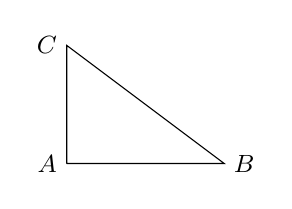
\begin{tikzpicture}[font=\small,x=5mm, y=5mm]

\draw (0,0)-- (4,0)--(0,3)--(0,0);

 \begin{scope}[left]
\node  at (0,3) {$C$};
\node  at (0,0) {$A$};
\end{scope}

\node[right]  at (4,0) {$B$};

\end{tikzpicture}
\end{center}
\end{multicols}

\emph{Procedura risolutiva}:
Dato che $\Area (ABC) =\dfrac{1}{2}\overline{AB}\cdot \overline{AC}$,
dobbiamo calcolare la lunghezza dei cateti.

Il dato $AC=\dfrac{3}{5}CB$ può essere scritto come: $AC=3x \wedge CB=5x$.
L'altro cateto si può calcolare con il teorema di Pitagora:
$AB=\sqrt{(5x)^2-(3x)^2}=\sqrt{25x^2-9x^2}=\sqrt{16x2}=4x$

Il perimetro è: $2p=4x+5x+3x=12x=120$ e da questa equazione ricaviamo 
$x=10$ da cui: $AB=40, BC=50, CA=30$

Da cui si ricava facilmente l'area: 
$\Area=AB \cdot AC \cdot \frac{1}{2} = 40 \cdot 30 \cdot \frac{1}{2} =600$
\end{soluzione}
